\begin{frame}
\frametitle{La realtà di interesse}
\setbeamercolor{block body}{bg=black!0}
\begin{block}{Modello teorico di estrazione del segnale dalla scansione}
\begin{figure}
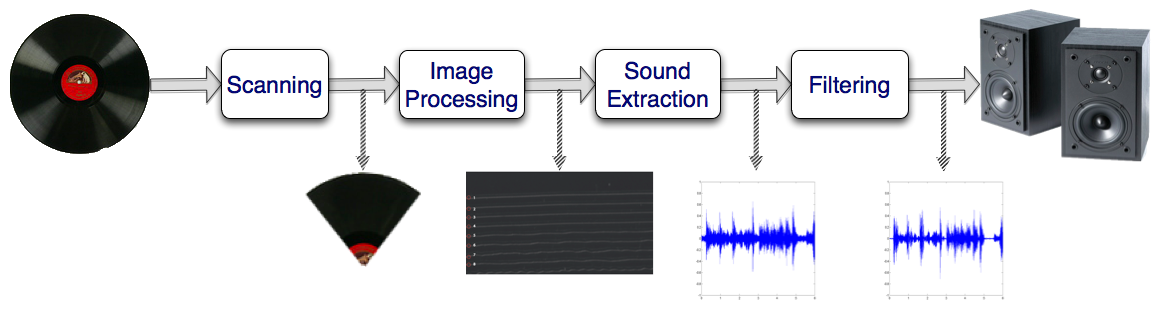
\includegraphics[width=1\textwidth]{immagini/block-scheme.png}
\end{figure}
\end{block}
\end{frame}

\begin{frame}
\frametitle{La realtà di interesse}
\begin{block}{Il processo di scansione: considerazioni preliminari}
Analisi preventiva per capire i problemi da affrontare:
\begin{itemize}
\item Scegliere la risoluzione adatta
\item Individuare la porzione della scansione con più informazione
%\item[*] individuare la porzione di disco meglio illuminata (discorsi su ottiche);
\item Come partizionare il disco?
\end{itemize}
\end{block}


\begin{block}{Il processo di scansione: cosa suggerisce la teoria?}
%Studio della letteratura per discriminare tra possibili scelte 
\begin{itemize}
\item Risoluzione 2400 dpi ottici
\item Non sempre banale la scelta della posizione corretta per la scansione
\item Scelte per il partizionamento varie (solitamente 4 fette)
\end{itemize}
\end{block}
\end{frame}

\begin{frame}
\frametitle{La realtà di interesse}
\begin{block}{L'elaborazione dell'immagine: la teoria}
\begin{columns}[t]
\begin{column}{6.5cm}
\begin{description}
\item[Ricerca del centro] Individuazione di un insieme di punti che permetta 
di stimare le coordinate del centro e il raggio
\item[Unwrap dell'immagine] Con i dati ricavati al punto precedente, si
opera una trasformazione da coordinate cartesiane a polari
\item[Crop dell'immagine] Eliminazione di porzione di immagine inutili o
``dannose''
\end{description}
\end{column}
\vline
\begin{column}{3.5cm}
\begin{figure}
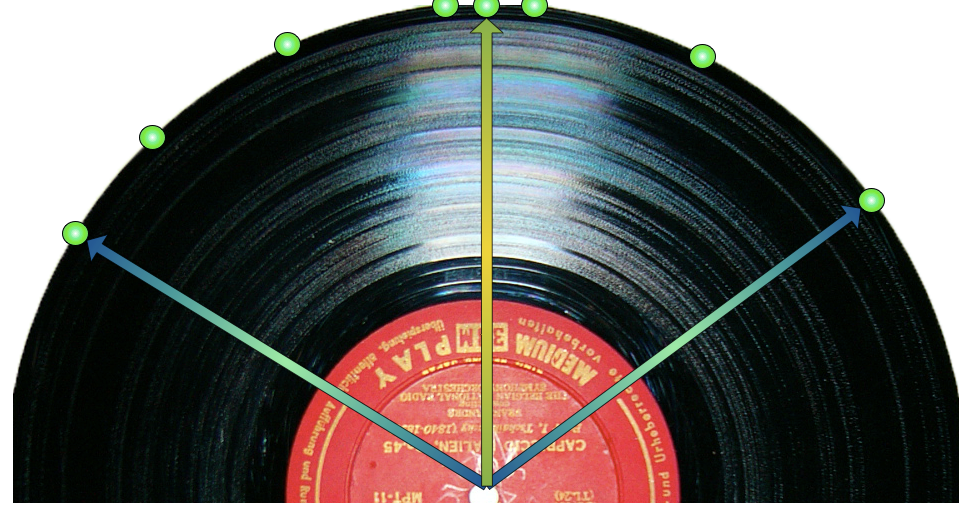
\includegraphics[width=0.5\textwidth]{immagini/center.png}\\
%\vspace{.2cm}
$\downarrow$\\
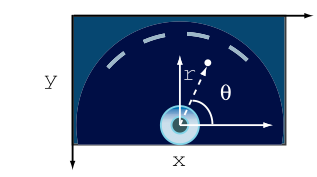
\includegraphics[width=0.5\textwidth]{immagini/cartesio.png}\\
$\downarrow$\\
\vspace{.2cm}
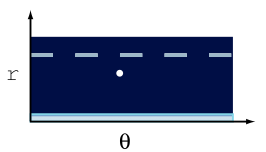
\includegraphics[width=0.5\textwidth]{immagini/polare.png}
\end{figure}
\end{column}
\end{columns}
\end{block}
\end{frame}

\begin{frame}
\frametitle{La realtà di interesse}
%\begin{block}{L'estrazione del suono: considerazioni preliminari}
%\'E stato necessario capire molto bene come mappare le variazioni presenti
%sul disco, in modo da effettuare una traduzione sensata e fedele.
%\end{block}
\begin{block}{L'estrazione del suono: cosa suggerisce la teoria}
\begin{columns}
\begin{column}{6.5cm}
\begin{description}
\item[Ricerca delle tracce] Si ricavano, dalle immagini elaborate, le coordinate
di inizio traccia
\item[``Inseguimento'' delle tracce] Si effettua un \emph{edge-detection}
intelligente, per ricavare il segnale
\item[Concatenzione delle tracce] Attraverso un'analisi della correlazione
tra le varie porzioni, si cercano sovrapposizioni e si giustappongono le 
tracce
\end{description}
\end{column}
\vline
\begin{column}{3.5cm}
\begin{figure}
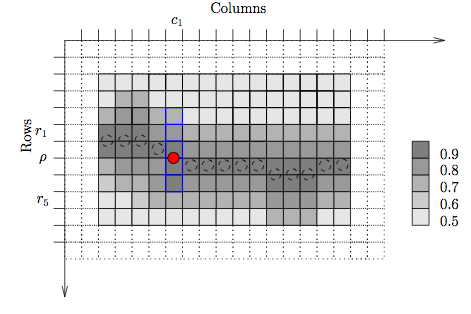
\includegraphics[width=0.7\textwidth]{immagini/track-following.png}
$$\downarrow$$
\vspace{0.2cm}
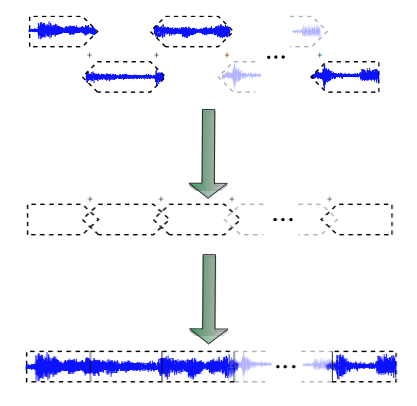
\includegraphics[width=0.7\textwidth]{immagini/concatenation.png}
\end{figure}
\end{column}
\end{columns}
\end{block}
\end{frame}
